\begin{question}
\noindent A UI/UX designer is working on a symmetric app icon. The current design, a triangle $T$ with vertices $A(1,2)$, $B(4,1)$ and $C(2,4)$, needs to be reflected in the line $y = x$ to create a mirrored version of the icon, $T'$.

\begin{center}
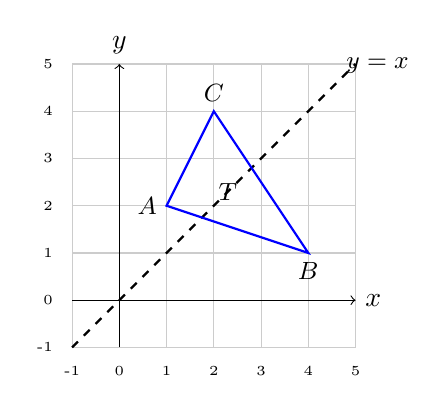
\begin{tikzpicture}[scale=0.6]
    \draw[step=1cm, gray!40, thin] (-1,-1) grid (5,5);
    \draw[->] (-1,0) -- (5,0) node[right] {$x$};
    \draw[->] (0,-1) -- (0,5) node[above] {$y$};
    \foreach \x in {-1,0,1,2,3,4,5} \draw (\x,-1.2) node[below,font=\tiny] {\x};
    \foreach \y in {-1,0,1,2,3,4,5} \draw (-1.2,\y) node[left,font=\tiny] {\y};

    \draw[dashed, thick] (-1,-1) -- (5,5);
    \node[above right, font=\small] at (4.6,4.6) {$y=x$};

    \draw[thick, blue] (1,2) -- (4,1) -- (2,4) -- cycle;
    \node[left, font=\small] at (1,2) {$A$};
    \node[below, font=\small] at (4,1) {$B$};
    \node[above, font=\small] at (2,4) {$C$};
    \node[font=\small] at (2.3,2.3) {$T$};
\end{tikzpicture}
\end{center}

\noindent Reflect triangle $T$ in the line $y = x$.

\noindent Write down the coordinates of the vertices of the image, $T'$.

\vspace{5cm}

\begin{flushright}
\answerplain{3}
\end{flushright}
\end{question}